\chapter{Background}


%%%%%%%%%%%%%%%%%%%%%%%%%%%%%%%%
%         Cosmic-ray
%%%%%%%%%%%%%%%%%%%%%%%%%%%%%%%%
\section{Cosmic-ray}

This section consists of historical discovery, from the origin
on this field of study until the latest impactful experiment.
Not only historical content, it also contains the physical
explaination with phenomenon that involving the CR reserch.

\subsection{History}
In 1909, the famous experiment that pioneer the study of CR has been
led by Theodor Wolf who take conduct the experiment of 
altitude variation by taking the apparatus to measure 
the rate of ionization from the ground to the top of 
the Eiffle Tower in Paris (\cite{gray1949cosmic}).
The result shown that there the ionizaiton rate was slightly
increase when the altitude is higher which gives the clues
that the origin of cosmic-rays was came from the outer space
rather than Earth's inner shell. \cite{EarlyCRGerman}

\begin{figure}[h!]
    \centering
        \subfloat[
            An early version schematic view of electrometer used by Thedor Wulf
            (\cite{EarlyCRGerman})
        ]{
            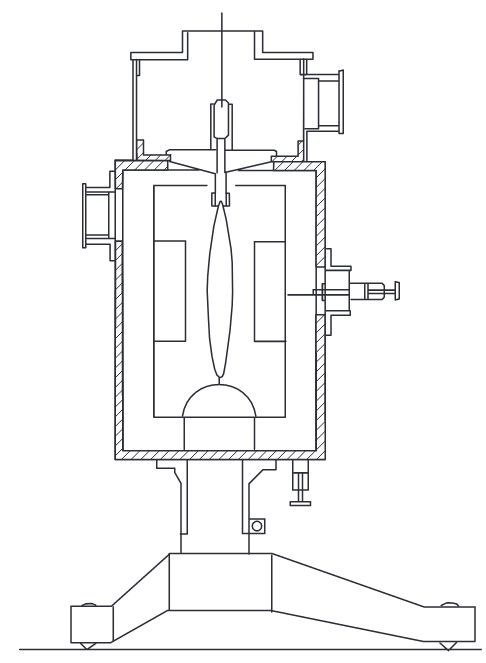
\includegraphics[width=0.35\textwidth]{content/background/figures/wulf_schema.png}
            }
        \hfill
         \subfloat[
            Ionizaiton rate from Victor Hess (left) and Werner
            Kolhörster (right)
         ]{
            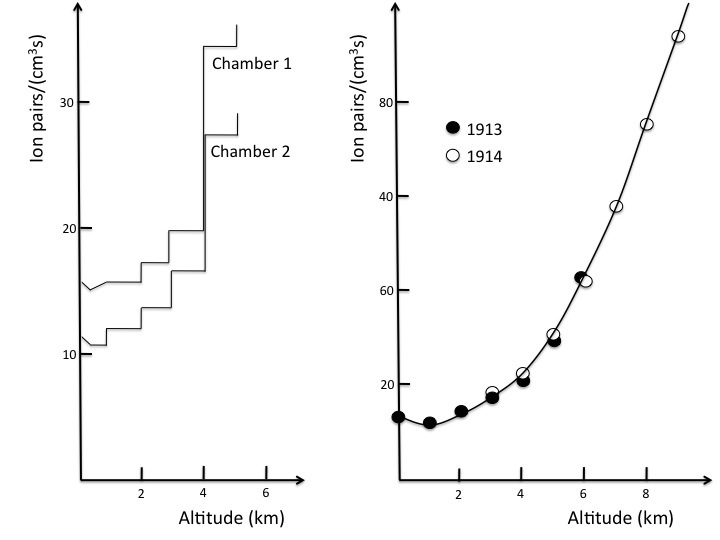
\includegraphics[width=0.6\textwidth]{content/background/figures/HessKol.jpg}
            }
        \caption{Wulf's apparatus and the ballon experimental results}
       \label{fig:xxx}
\end{figure}


However, the experiment of measuring the affect of altitude
variation with a tiny altitude scale comparing to the Earth's
atmosphere would not enough to consolidate the theory.
In the same year, the ballon with a similar instrument has
been released up to 1.3 kilometers by Karl Bergwitz to put 
more weight on the first experiment. They found that the 
ionization has increased by a quater comparing to ground level 
(\cite{de2014atmospheric}).
Three years later, suicidal investigation was conducted by 
an Australian gentleman who brought the detector and himself
to fly with the balloon.
His name is Victor Hess, people might have no doubt why this
name went so famous because he risk his life with the experiment 
and he was flying over 5 kilometers above the ground (\cite{hess1912beobachtungen}).
Definitely, the result is strongly significant and impactful
to the astrophysical research community. Risking life  
In 1914, Werner Kolhörster repeated the balloon experiment 
with higher altitude which around 9 kilometers from the 
sea level and the ionizaiton rate still does increase when 
the ballon flown higher. This emphasize that the source of 
those ionizing ray came from Earth's upper atmosphere
or the outer space.

\begin{figure}[h!]
    \centering
        \subfloat[Main  points  where  CR  intensities  were  measured  during  eight Compton expeditions in 1932]{
            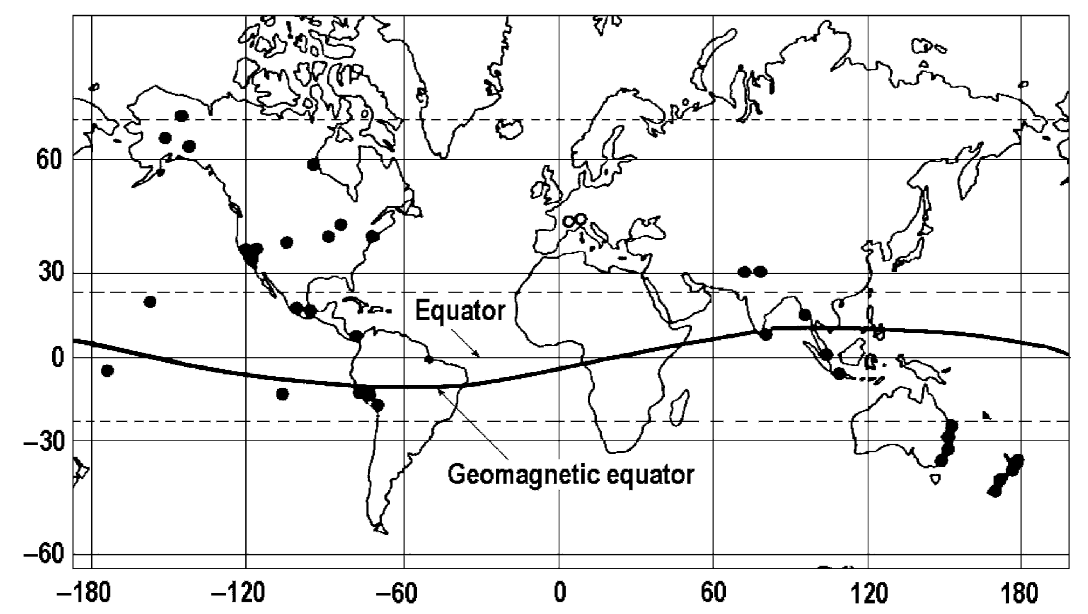
\includegraphics[width=0.62\textwidth]{content/background/figures/clay_geographical.png}
            }
        \hfill
         \subfloat[
            The Pb-shielded ionization chamber, 
            organized by Compton (\cite{text_cr_geomagnetic_effect})    
         ]{
            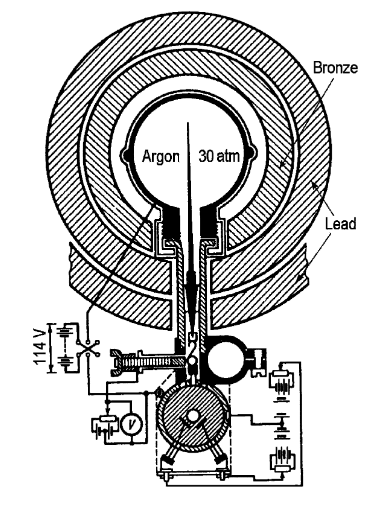
\includegraphics[width=0.32\textwidth]{content/background/figures/compton_pb_shield.png}
            }
        \caption{Clay Experiment of geographical variation}
       \label{fig:clay_cr_ship}
\end{figure}

Not only the altitude variable that related to the 
intensity of the CRs, but the geographic location of the 
obvervation also does affect to the measurement.
The first experiment has done done John Clay who
sailed the ship across the ocean from Holland to Java
(\cite{Clay1927,Clay1928}). The geographical locations 
that used to measure the CR intensities and the 
apparatus schematicical draft is shown in Figure
\ref{fig:clay_cr_ship}. The result shows that
the further from equator, the higher CR intensity.
Another exploration for the geographic variation was 
done by John Compton in the following five years.
He basically sailed the ship from the Sydney (northern hemisphere)
to Vancouver (the southern hemisphere) for various season
during 1936 to 1937 back and forth (\cite{compton1937cosmic}).
The Figure \ref{fig:comptonship} demonstrates the 
latitude variation and the seasonality effects of the 
multiple trips from the experiment.

\begin{figure}[h!]
    \centering
    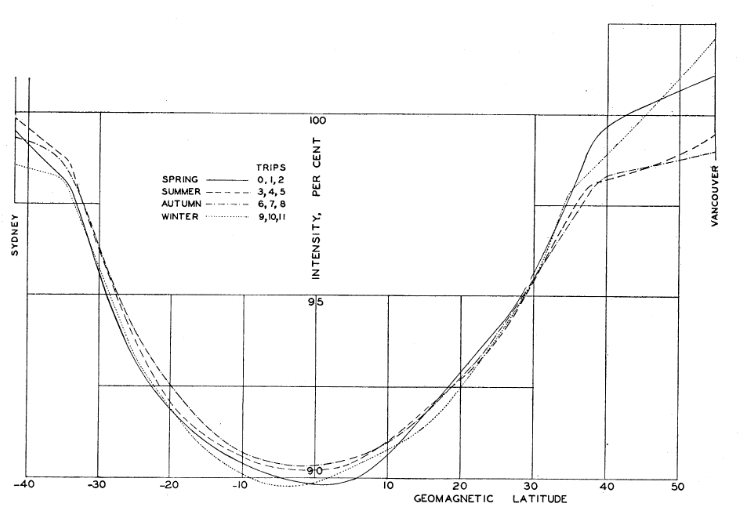
\includegraphics[width=\textwidth]{content/background/figures/compton_sail_1937.png}
    \caption{Latitude variation for various seasons (\cite{compton1937cosmic})}
    \label{fig:comptonship}
\end{figure}
	
The first interpretation study from the discovery has been
done by Carl Störmer. The explaination of the CR's altitude variation
came from the trajectory of CR particles due to geomagnetic field
(\cite{stormer1934critical}). In that period, the topic of 
geomagnetic field and the effects of CRs was quite famous.
Another impactful study of the CRs trajectory and the relevant
of Earth's magnetic field was conducted by Bruno Rossi
for predicting an asymmetry of the East-West distribution
of CR spectrum because the primary CRs does have a positive or
negative charge then the cyclic moving direction of the 
particle was induced by Lorentz force where the direction of 
the Earth's magnetic field could be identified to determine the
direction of the charged particles (\cite{rossi1941cosmic}).

The ground based detector is a great option for 
detecting the CRs where it include primary and secondary CRs.
However, investigating the primary CRs is a challenging topic
for ground based detector especially for low energy particles.
Another interesting option to inspect the asymmetry of 
East-West could be done by using space based detector 
that orbiting around the Earth's at some radius in the
higher altitude and definitely it would face a lower 
atmospheric density which consider to be an interesting 
choice to study the CRs with a lower effects of atmospheric
interaction. In 2008, \textit{Fermi} Large Area Telescope (LAT)
has been launched to observed $\gamma$-ray and
lightweight lepton particles which basically are electron
and position. The East-West effects from geomagnetic
induction was also emphasized by \textit{Fermi}-LAT.


\subsection{Physical properties}
CRs are high energy particles that propagating through
the space. The momentum of the particles came from
various acceleration mechanism base on where it from 
such as supernovae, active galactic nuclei, quasars 
and gamma-ray bursts. The composition of CRs consists of
90\% protons, 8\% alphas and other nuclei of heavier
elements (\cite{CRComposition2017}). Experimentally,
many observations indicate that the spectrum of CRs 
for all particles and individually does follow the 
power law in rigidity (momentum per charge) with a specific spectral index depends on 
their energy range. Theoretically, the observed spectrum
with a broad energy range would represented the superposition
of arrival CRs with a diverse producers where each producer
has their own specific character which is spectral index.
By the end of the day, it is barely possible to distinguish
the origin of CR particles one by one. Then it is more 
plausible to provenance the origin of CR particles in the 
macroscale rather than inspecting in the microscale.




\begin{figure}[h]
    \centering
    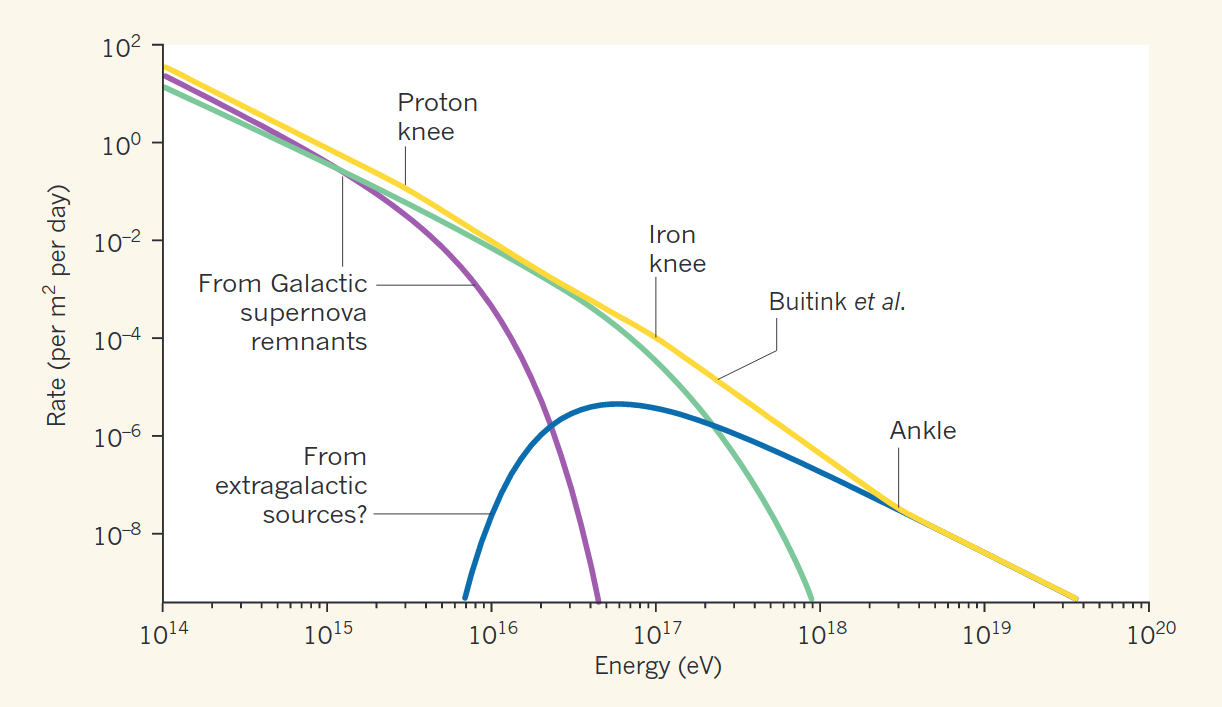
\includegraphics[width=\textwidth]{content/background/figures/andrew_superposition.png}
    \caption{Superposition of CR spectrum (\cite{taylor2016_crspectrumsuperposition})}
    \label{fig:cr_superposition}
\end{figure}

As mentioned in an early paragraph, each souce of CR does reflect their
own specific spectral index in the arrival CR spectrum.
In order to validate the theoritical assumption, putting 
the simulation or calculation of each sources and check
with the real data does compliment experimental observations.
The superposition of various sources that yield a 
discontinuity of the spectral indices has been exploided
in some energy ranges. Two well known breaking points 
are knee and ankle where it located in the energy order 
around $10^{15}$ eV and $10^{18}$ eV sequentially.
Approximately, the rate to find one particle at knee
is around one particle per square meter per year and 
the possibility that the apparatus could detect the particle
in energy at ankle point is roughly one particle per 
kilometer per year. Figure \ref{fig:cr_superposition} illustrate
the concept of superposition from various sources and 
yield the arrival CR spectrum with a breaking spectral indices. 

Not only the below ankle energy that has an interesting
properties, but the CR that has energy beyond the ankle energy
also has an identical properties. It knowns as "ultra-high
energy cosmic rays" (UHECR). One interesting point is that it 
does not that far from ankle in term of rigidity magnitude
which higher around 1 or 2 order of magnitude. The widely known 
explaination why it could not go so far is the
Greisen–Zatsepin–Kuzmin limit (GZK limit).
The theory provides the description why it the UHECR
could not propagte though the space but please note that
some sources still could produce such a UHECR but the main
issue here it the space does not empty. It contains some 
intermediate matter or dust and the microwave background radiation
which it is believed that it came from the residue of the 
Big Bang or some greate explosion or expansion of the space that 
human never saw it (at least in the human lifetime).
The main calculation of the CR kinetic energy limit from GZK 
was considered only proton particles and the main interaction
that makes it stop is basically from the interaction with 
microwave background radiation that almost perfectly
isotropically progating in the space with an order of 
traveling proton around hundred light years in the space
(\cite{gzk_cr_limit}). The way of this kind of intereaction 
not only does slow down the CR proton by producing 
neutral pion where it mostly decay into a pair of $\gamma$-rays
but it could also yield a neutron with 
a charged pion. Hence, it is also answer why we could 
see such a high energy neutron that does not only 
produced in the sky (shower effects) albeit it does not
has any charge to be accelerated in the famouse 
acceleration mechanism such as shock acceleration.

The types of CRs could be divided into two kinds based on
how they was produced which are
\begin{enumerate}
    \item \textbf{Primary cosmic rays}: they mostly be produced from the
    Solar system, somewhere in the Milky ways, extragalactic sources
    and many more. When they interact with the Earth's atmosphere,
    with the hadronic interaction with the air molecules,
    they produce the secondary CR particles.
    \item \textbf{Secondary cosmic rays}: as mentioned in collapsing of the  
    primary CRs, secondary CRs consists of many particles
    from lightweight leptons to medium weight leptons and 
    from mesons to hadron particles as well. The interaction
    of the proton with the atmospheric molecule looks simple 
    but the precise calculation from derivation is extremely complicate 
    since there are endless possibility of the (Feynman) path that 
    also produce another products with a certain probability.
    By the end of the day, we definitely got a few certains 
    of particles from their likelihood of the occurence from 
    the collision which mainly are electrons, positions, muons,
    pions and photons as demonstrates in Figure \ref{fig:cr_shower}.
\end{enumerate}

\begin{figure}[h]
    \centering
    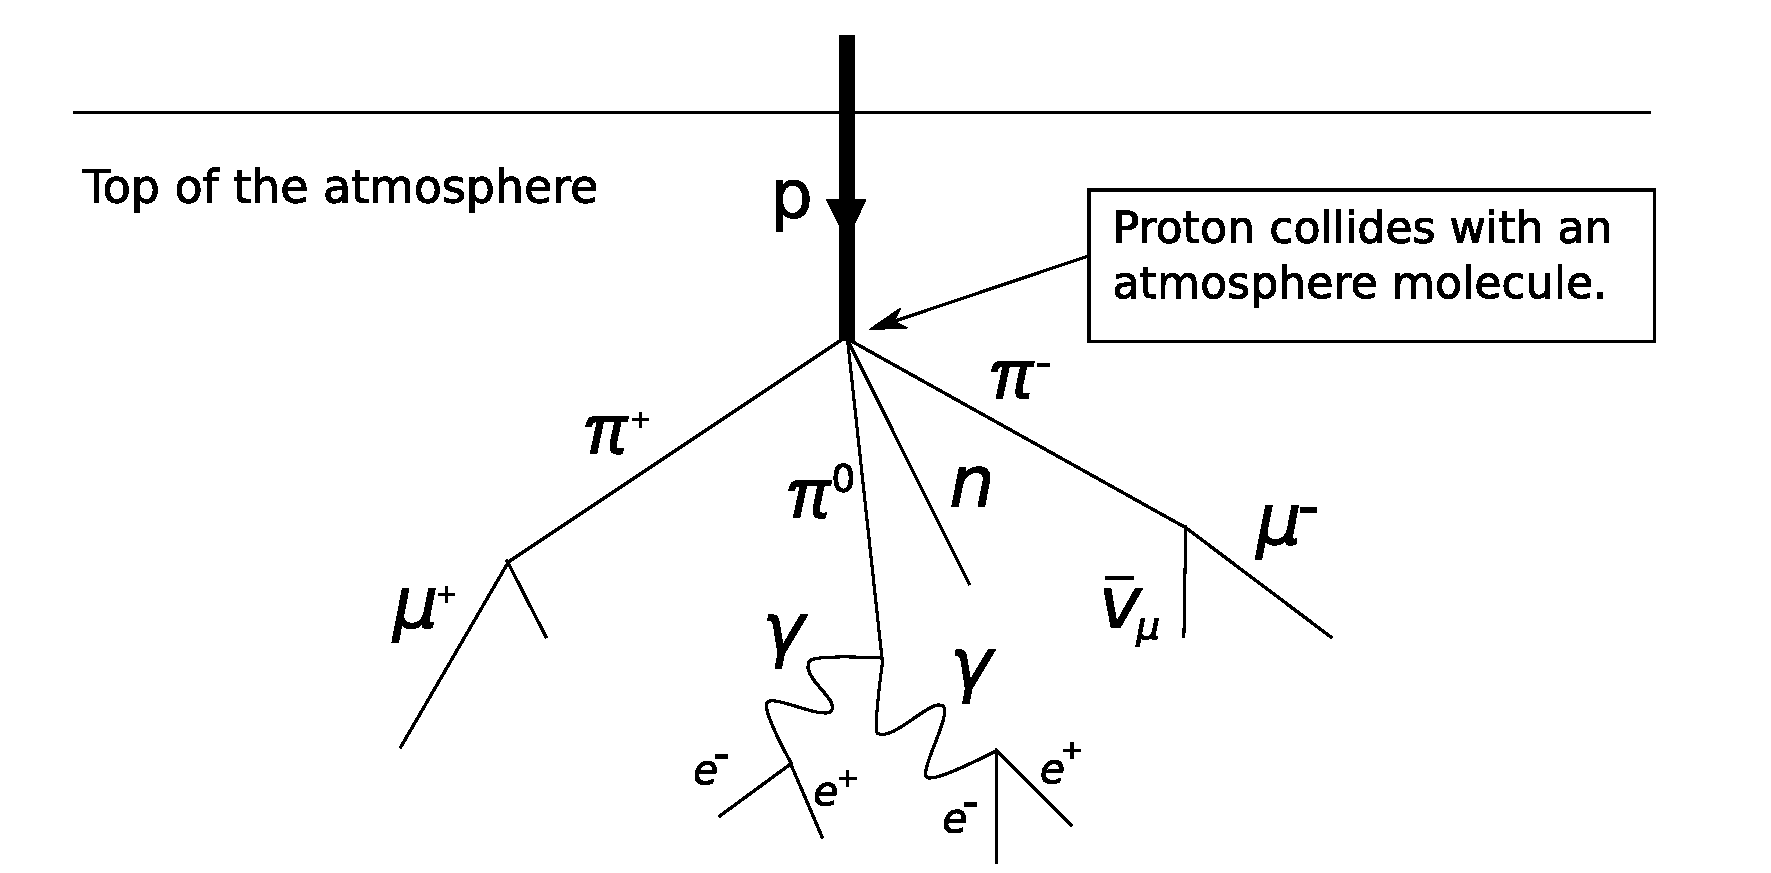
\includegraphics[width=\textwidth]{content/background/figures/Atmospheric_Collision.pdf}
    \caption{Cosmic rays shower from collision of primary CR with the atmospheric molecule
    }
    % 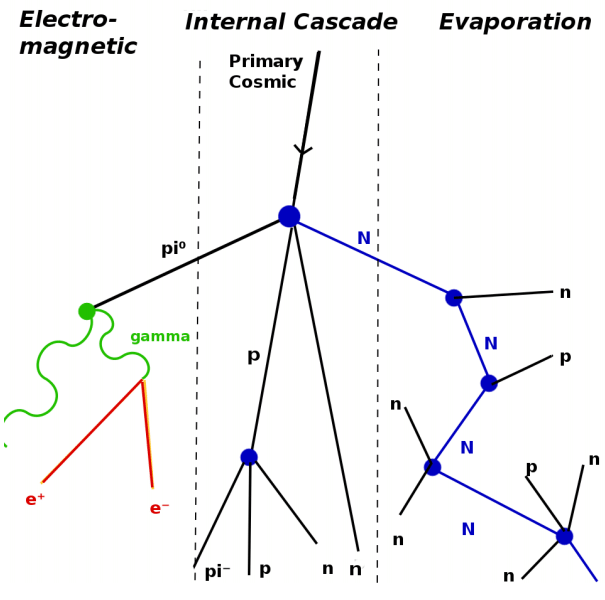
\includegraphics[width=0.7\textwidth]{content/background/figures/cr_shower2.png}
    % \caption{Cosmic rays shower from collision of primary CR with the atmospheric molecule.
    % Image taken from \cite{cr_shower_img}
    % }
    \label{fig:cr_shower}
\end{figure}


\subsection{$\gamma$-ray production}

The production of $\gamma$-ray particles happens all the 
time. It is mandatory to understand how a photon could 
gain a very high momentum from the nature. The procedure 
to acquire all those kinetic energy is quite different from how
a charged particle obtains their momentum because a 
charged particle could earn their kinetic energy during 
 their trip of propagating through the space with a 
Lorentzian force. The $\gamma$-rays mostly have only one 
chance to pick their kinetic energy and it happens when it 
was produced bacause it is barely interact with any other 
particles in the space especially high energy $\gamma$-ray.
The scenarios that makes photon hold a high energy are 
listed in the following bullets.

\subsubsection{Mechanism of $\gamma$-ray producing}

\begin{itemize}
    \item \textbf{Decaying of unstable matter}:
    Radioactive decay is one of the most well known
    phenomena for the $\gamma$-decay mode. One example 
    of the heavy ion decay is the cobalt-60. It decays 
    into excited state of nickle as

    \ch{27^{60}Co -> 28^{60}Ni^{*} + e- + $\bar{\nu}$ + $\gamma$},

    then the excited nickle decay another $\gamma$-ray
    to make it to the stable state

    \ch{28^{60}Ni^{*} -> 28^{60}Ni + $\gamma$ }.

    The famous decay of a lower level from a small 
    nuclei that consists of two quarks called "meson".
    To be more precise, it is known as the pion decay.
    The path diagram is demonstrated in Figure \ref{fig:neutral_pion_decay}
    where the neutral pion from the collision process that
    interact via Yukuwa's interaction. The neutral pion itself
    does not stable then it would have a short amount of lifetime 
    before it dominately decays into two high energy photons.
    \begin{figure}[h]
        \centering
        \begin{tikzpicture}
    \begin{feynman}
    \vertex (a);
    \vertex [below= of a] (b);
    \vertex [left= of a] (p1) {\(u\)};
    \vertex [left= of b] (p2) {\(\bar{u}\)};
    \vertex [right= of a] (q1) {\(\gamma\)};
    \vertex [right= of b] (q2) {\(\gamma\)};
    
        \diagram* {
            (p1) -- [fermion] (a) ,
            (a) -- [fermion] (b),
            (b) -- [fermion] (p2) ,
            (a) -- [photon] (q1),
            (b) -- [photon] (q2),
        };
    \end{feynman}
\end{tikzpicture}
% \begin{tikzpicture}
%     \begin{feynman}
%     \vertex (a);
%     \vertex [below= of a] (b);
%     \vertex [left= of a] (p1) {\(d\)};
%     \vertex [left= of b] (p2) {\(\bar{d}\)};
%     \vertex [right= of a] (q1) {\(\gamma\)};
%     \vertex [right= of b] (q2) {\(\gamma\)};
    
%         \diagram* {
%             (p1) -- [fermion] (a) ,
%             (a) -- [fermion] (b),
%             (b) -- [fermion] (p2) ,
%             (a) -- [photon] (q1),
%             (b) -- [photon] (q2),
%         };
%     \end{feynman}
% \end{tikzpicture}

% \begin{tikzpicture}
%     \begin{feynman}
%         \vertex (a);
%         \vertex [above right= of a] (b);
%         \vertex [below right= of a] (c);
%         \vertex [left= of a] (p1) {\(\pi^0\)};
%         \vertex [right= of b] (q1) {\(\gamma\)};
%         \vertex [right= of c] (q2) {\(\gamma\)};

%         \diagram* {
%             (p1) [particle] -- [scalar] (a),
%             (a) -- (b),
%             (a) -- (c),
%             (b) -- (c),
%             (b) -- [photon] (q1),
%             (c) -- [photon] (q2),
%         };
%     \end{feynman}
% \end{tikzpicture}
        \caption{Feynman's diagram of neutral pion decays into two $\gamma$-rays}
        \label{fig:neutral_pion_decay}
    \end{figure}
    Definitely, neutral pion also could yield one $\gamma$-ray
    and a pair of lightweight leptons, a couple 
    pair of lightweight leptons or even just a pair 
    of lightweight leptons and much more as long as it 
    conserve the momentum, energy and the quantum numbers.
    The main reason why the majority of their decaying process
    does yield only photons because the scattering amplitude
    as the Figure \ref{fig:neutral_pion_decay} does hold a branching
    ratio around 0.98823 and the rest of them is 
    smaller than 1\%. Another interesting property of this 
    decay mode is the momentum vector of their pair $\gamma$-ray
    hold an opposite direction with the same amplitude in the 
    reference frame.

    \item \textbf{electron–positron annihilation}:
    In the universe, there are some probability of the electron and 
    position was forced to face each other by some chance from
    the electromagnetic force or randomly found each other.
    The intereaction when they facing each other dominate by 
    electromagnetic interaction and definitely require a photon
    as a mediator to allow them talk to each other in quantum 
    electro dynamics point of view. Definitely, there is a change 
    when those pair of leptons decide to annihilate into high energy photons
    without runing any physical laws. Nevertheless, other kind of
    a pair of leptons like muon technically could deforms into two
    photons with much higher energy because their rest mass is higher.
    Surely, a pair of Tau is also allow to produces a pair of photons.
    However, the lifetime of those medium-weight and heavy-weight leptons
    could not last that long to survive in practical. The simplest 
    Feynman's path of annihilation of leptons into a pair photons 
    is illustrated in Figure \ref{fig:lepton_annihilation} from light 
    to heavy leptons sequentially.

    \begin{figure}[h!]
        \centering
            \subfloat[
                Lightweight leptons
            ]{
                \begin{tikzpicture}
\begin{feynman}
\vertex (a);
\vertex [below= of a] (b);
\vertex [above left= of a] (p1) {\(e^{-}\)};
\vertex [below left= of b] (p2) {\(e^{+}\)};
\vertex [above right= of a] (q1) {\(\gamma_1\)};
\vertex [below right= of b] (q2) {\(\gamma_2\)};

    \diagram* {
        (p1) -- [fermion] (a) ,
        (a) -- [fermion] (b),
        (b) -- [fermion] (p2) ,
        (a) -- [photon] (q1),
        (b) -- [photon] (q2),
    };
\end{feynman}
\end{tikzpicture}
            }
            \hfill
            \subfloat[Mediumweight leptons]{
                \begin{tikzpicture}
    \begin{feynman}
    \vertex (a);
    \vertex [below= of a] (b);
    \vertex [above left= of a] (p1) {\(\mu^{-}\)};
    \vertex [below left= of b] (p2) {\(\mu^{+}\)};
    \vertex [above right= of a] (q1) {\(\gamma_1\)};
    \vertex [below right= of b] (q2) {\(\gamma_2\)};
    
        \diagram* {
            (p1) -- [fermion] (a) ,
            (a) -- [fermion] (b),
            (b) -- [fermion] (p2) ,
            (a) -- [photon] (q1),
            (b) -- [photon] (q2),
        };
    \end{feynman}
    \end{tikzpicture}
            }
            \hfill
            \subfloat[
                Heavyweight leptons
             ]{
                \begin{tikzpicture}
    \begin{feynman}
    \vertex (a);
    \vertex [below= of a] (b);
    \vertex [above left= of a] (p1) {\(\tau^{-}\)};
    \vertex [below left= of b] (p2) {\(\tau^{+}\)};
    \vertex [above right= of a] (q1) {\(\gamma_1\)};
    \vertex [below right= of b] (q2) {\(\gamma_2\)};
    
        \diagram* {
            (p1) -- [fermion] (a) ,
            (a) -- [fermion] (b),
            (b) -- [fermion] (p2) ,
            (a) -- [photon] (q1),
            (b) -- [photon] (q2),
        };
    \end{feynman}
    \end{tikzpicture}
            }
            \caption{Major lepton annihilation path diagram}
           \label{fig:lepton_annihilation}
    \end{figure}

    \item \textbf{Synchrotron radiation\& Bremsstrahlung radiation}:
    The phenomena of turning momentum direction of charged particle
    or accelerate into another direction shares a similar
    description. Conservation of momentum has come into place when 
    considering the bending charged particle that would emit the
    photon. Regarding the incoming direction of a charged particle 
    and then turning it direction by $\pi/2$ radians. The question
    that comes into mild is where does those initial momentum in an 
    incoming direction does since the momentum is conserved along 
    the cartesian direction, not only the magnitude. Now the clue is 
    here, they have to emit the photon to converse the momentum of 
    the system.
    
    Let walk through the first example called
    synchrotron radiation. Keeping some charged particle circulating 
    around the donut-like apparatus have some cost to pay to make 
    them stay without escaping the tunnel. Unquestionably, draging
    some moving particle circulating around some point requires a
    centripedal force. In this case, applying electromagnetic force
    without toucing it would yield a radiation called synchrotron emission.

    The second mechanism is Bremsstrahlung, where a charged particle 
    or typically an electron moving path close to some opposite charged 
    particle or typically a proton. The explaination from Coulomb's law
    would cover this scheme for the definition that the force is 
    inverse proportional to the distance between two charges. Then 
    moving pass by an opposite charged particle does induced the electron
    bending and emit the photon because the explained reason from the 
    previous paragraph. This mechanism happens when an CR electrons 
    moving through the matter of Sun's chronosphere and interact with 
    a positive charged and produce some high energy photon but usually 
    it produce in the X-ray energy range.


\end{itemize}



% decel & ac cel
\subsubsection{Mechanism of $\gamma$-ray gaining momentum}

Even though, $\gamma$-ray usually does not prefer
to talk to another fundamental particles because
scattering amplitude of their interaction is pretty 
low. Nonetheless, there are some scenarios that $\gamma$ could 
gain more kinetic energy and losing their kinetic energy 
when they traveling in the universe.

\begin{itemize}
    \item \textbf{Inverse Compton scattering}
    The scattering of a photon (massless particle) with an electron 
    (massive particle) could occur during their trip. Equation \ref{eq:inv_compton} 
    demonstrate the symbolic relation of the scattering with the 
    electromagnetic interaction and yield the same particles as an 
    incoming particles.

    \begin{equation}
        e^-\gamma \rightarrow e^-\gamma
        \label{eq:inv_compton}
    \end{equation}

    Interaction between an electron and a photon could 
    make them converting the momentum via the scattering
    processs. Since the system momentum has to be conserved,
    then there will be one losing momentum and another one gaining 
    momentum or kinetic energy. Suppose one photon is traveling 
    and hit electron or a charged particle, it could transfer the 
    kinetic energy to the particle and their wavelength will be 
    longer. In another word, it is lossing the kinetic energy.
    On the other hand, this scenario could happen in the opposite way.
    There is situation when a high energy electron interacting with 
    the photon and turn over it kinetic energy to the photon. After that,
    a photon could gain more kinetic energy during their trip. 
    The latter scenario is called "Inverse Compton Scattering".
    The most likelihood choice of interaction of the scheme could be 
    represented in Feynman's path as in Figure \ref{fig:compton_feynman}.

    \begin{figure}[h!]
        \centering
            \subfloat[First branch]{
                \begin{tikzpicture}
    \begin{feynman}
    \vertex (a);
    \vertex [right= of a] (b);
    \vertex [below left= of a] (p1) {\(e^{-}\)};
    \vertex [above left= of a] (q1) {\(\gamma_1\)};
    \vertex [below right= of b] (p2) {\(e^{-}\)};
    \vertex [above right= of b] (q2) {\(\gamma_2\)};
  
      \diagram* {
        (a) -- [fermion, edge label'=\(\)] (b) ,
        (q1) -- [photon, momentum] (a) ,
        (p1) -- [fermion] (a),
        (b) -- [photon, momentum] (q2),
        (b) -- [fermion] (p2),
      };
      \vertex [below= 0.5em of a] {\(\)};
      \vertex [below= 0.5em of b] {\(\)};
    \end{feynman}
  \end{tikzpicture}
                }
            \hfill
             \subfloat[
                Second branch
             ]{
                \begin{tikzpicture}
    \begin{feynman}
    \vertex (a);
    \vertex [right= of a] (b);
    \vertex [below left= of a] (p1) {\(e^{-}\)};
    \vertex [above left= of a] (q1) {\(\gamma_1\)};
    \vertex [below right= of b] (p2) {\(e^{-}\)};
    \vertex [above right= of b] (q2) {\(\gamma_2\)};
  
      \diagram* {
        (a) -- [fermion, edge label'=\(\)] (b) ,
        (q1) -- [photon, momentum] (b) ,
        (p1) -- [fermion] (a),
        (a) -- [photon, momentum] (q2),
        (b) -- [fermion] (p2),
      };
      \vertex [below= 0.5em of a] {\(\)};
      \vertex [below= 0.5em of b] {\(\)};
    \end{feynman}
  \end{tikzpicture}

                }
            \caption{Trivial Feynman's path of (Inverse) Compton scattering}
           \label{fig:compton_feynman}
    \end{figure}
\end{itemize}




\subsubsection{$\gamma$-ray production plants}



\begin{itemize}
    \item \textbf{Supernova ramnants (SNRs) and molecular cloud}: 
    The supernova explosion is a huge expansion from that approximately
    expanding as a spherical shell that sweep the inter stellar medium (ISM)
    and decelerate at some radius after the enlargement. The kinetic 
    energy that transfer from the momentum in the radial axis was 
    modeled and belived to be the kinetic energy of the cosmic ray particles.
    There are three major processes that involves in this phenomenon which 
    are nuclear pion production, nonthermal electron bremsstrahlung, and Compton scattering
    (\cite{cr_from_snr_2013}). Last but not least, the shock acceleration
    could play an important role for this phenomenon.

    \item \textbf{Diffused $\gamma$-ray emission from galactic plane}:
    One of the bright source that does not locate too far from our teritory
    is the galactic plane. The first reasonable explaination is the 
    distance of the productive objects does not far from Earth comparing 
    to other extragalactic sources. In addition, there are many interesting 
    CR sources in our galaxy. It might be pulsar, some flare of the 
    event of an explosion and so on. The plot that shows the brightness
    of the galactic plane comparing to the outer space is shown in 
    Figure \ref{fig:gamma_galac_plane}.

    \begin{figure}[h]
        \centering
        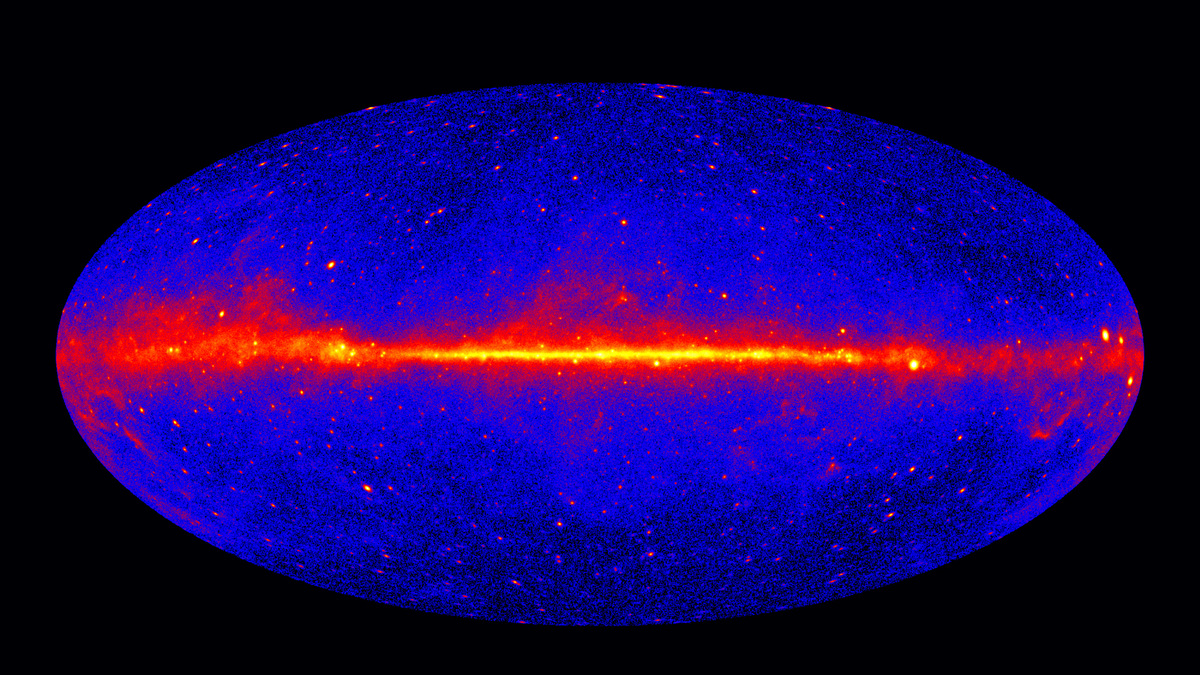
\includegraphics[width=\textwidth]{content/background/figures/Fermi_5_years.jpg}
        \caption{Intensity of $\gamma$-ray $>$ 1 GeV in galactic coordinate (Image credit: NASA/DOE/\textit{Fermi} LAT Collaboration)}
        \label{fig:gamma_galac_plane}
    \end{figure}

    \item \textbf{Pulsar and Active Galactic Nucleus (AGN)}: 
    Another source of the brightness in Figure \ref{fig:gamma_galac_plane}
    is the bright dots with a different solid angle width in the sky.
    The majority of those spots consists of $\gamma$-ray from 
    pulsar's periodic emission and AGN or extremely luminous AGN
    namely "Quasar". The cycle of the lighthouse effects from pulsar 
    is very robust as in the scale of atomic clock. Both of them 
    has a very high magnetic field strength. Emissive photons from 
    those sources would be a very high energy due to the accelation 
    of a charged particle near magnetic poles or the outer.


    \item \textbf{Earth's limb $\gamma$-ray production}:
    The closest $\gamma$-ray source is our Earth's atmosphere.
    To be more precise, the Earth's upper atmosphere is super bright 
    in $\gamma$-ray exposure. The main reason that cause the shining 
    of Earth's limb does came from the collision of the CR's massive
    particle such as protons and alphas. The interaction of those high 
    energy CR massive particles yield many more particles and main 
    contribution of the $\gamma$-ray dazzling came from the neutral pion
    decay which is the product from the collision process.

\end{itemize}



%%%%%%%%%%%%%%%%%%%%%%%%%%%%%%%%
%         Fermi-LAT
%%%%%%%%%%%%%%%%%%%%%%%%%%%%%%%%
\section{\textit{Fermi} Large Area Telescope (LAT)}
One of the famous space telescope that does see the sky in the 
visible wavelength is \textit{Fermi} Large Area Telescope (LAT).
Formerly, it was called Gamma-ray Large Area Space Telescope (GLAST).
The mission of the satellite is to collect high energy photon data 
or $\gamma$-ray and it technically could detect the lightweight
lepton particles namely electron and position.
The orbiting radius is around 550 kilometers
from the sea level. It is designed for observing the full-sky in 
$\gamma$-ray region. It also attach the Gamma-ray Burst Monitor (GBM) to study gamma-ray
bursts for seeking an exotic event. The telescope was launched in 
11 June 2008 at 16:05 UTC or 21:05 Bangkok time by abroading with 
Delta II 7920-H rocket.


\subsection{Overview}

\begin{figure}[h]
    \centering
    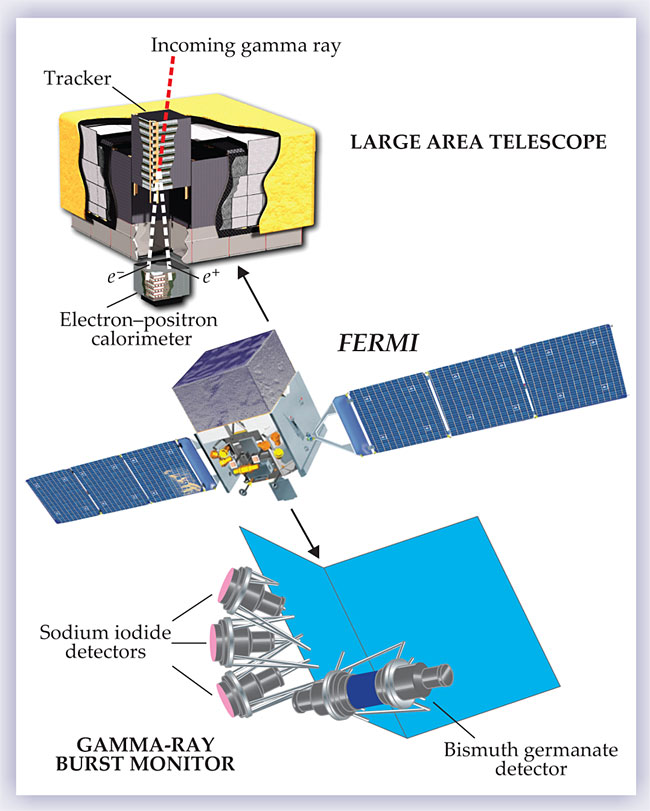
\includegraphics[width=0.6\textwidth]{content/background/figures/fermi_instrument.jpeg}
    \caption{Main components of \textit{Fermi}-LAT (Image taken from \cite{fermi_lat_instrument_first_year})}
    \label{fig:fermi_main_components}
\end{figure}
According to Figure \ref{fig:fermi_main_components},
each components of the $Fermi$ telescope was designed for a purpose since there 
is no ideal detector module that could detect kind of particles.
There are two main parts where the first part if the major component 
called Large Area Telescope (LAT) for detecting the $\gamma$
-ray and the second part is Gamma-ray Burst Monitor (GBM) for seeking 
an interesting event in the sky. In fact, both of them does detect 
the $\gamma$-ray but in the different energy scale. LAT is the main 
component where it detect the $\gamma$-ray in a few dozen of GeV 
up to a digit of TeV. For GBM part, the visible photon energy 
for them is around 8 keV to 40 MeV. The GBM consists of two 
sub components which are sodium iodide detector for low-energy photons
(8 keV to 1 MeV) and bismuth germenate detector for high-energy photons 
(0.2 MeV to 40 Mev). GBM detectors distribute around 
the telescope to be a closed circuit camera and looking for a flare 
of the $\gamma$-ray. The actual purpose of GBM is not a detector 
for collecting a high quality data but it is attached in the spacecraft 
to assist the LAT for mainly looking at an interesting events that could 
produce a huge amount of $\gamma$-rays. The content in this chapter 
will deep down into more detail of LAT in depth and would not provide 
more detail of GBM.

\subsection{Large Area Telescope (LAT)}


\begin{figure}[h]
    \centering
    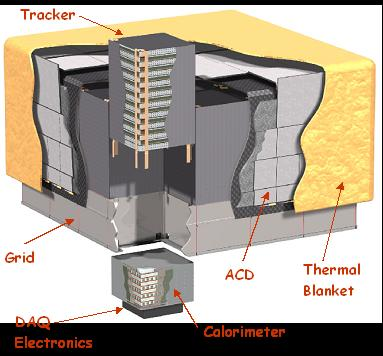
\includegraphics[width=0.6\textwidth]{content/background/figures/LATStructure.jpg}
    \caption{Instrument structure (Image taken from https://fermi.gsfc.nasa.gov)}
    \label{fig:fermi_lat_structure}
\end{figure}

LAT consists of tracker (TKR) module for tracing the incoming photon,
calorimeter (CAL) for measuring the kinetic energy after the particle 
has been passed through the tracker because a charged particle 
interact with the CAL and dissipate since it enter the module
and anti-coincidence Detector (ACD) for rejecting the background 
signal. The last part is the on-boarding data acquisition (DAQ)
module for investigating the particle's footprint and digitize
the signal.


\begin{figure}[h]
    \centering
    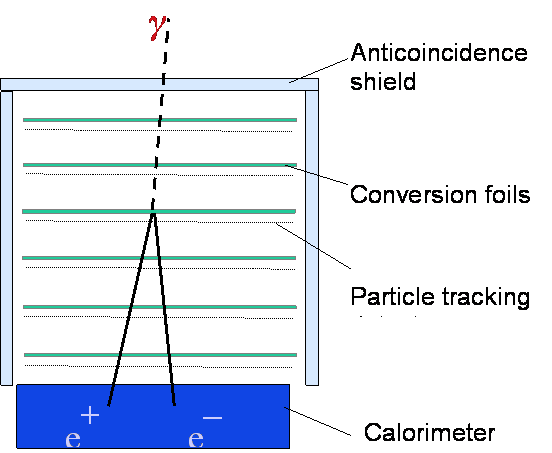
\includegraphics[width=0.6\textwidth]{content/background/figures/LAT_layers.png}
    \caption{Schematic structure of the LAT (Image taken from https://fermi.gsfc.nasa.gov)}
    \label{fig:fermi_lat_layers}
\end{figure}




\subsubsection{Tracker}
Higher energy photon or $\gamma$-ray talk to the LAT by converting the
kinetic energy into a pair of lightweight leptons or e$^{+}$e$^{-}$ pair.
The converter-tracker has 16 planes of a large atomic numbers for 
making the incident $\gamma$-ray convert into a pair of e$^{+}$e$^{-}$
as demonstrated in Figure \ref{fig:fermi_lat_layers}. After that, 
a pair of leptons would leave a footprint as an electromagnetic induction 
in particle tracker where it sensitive for the moving charge particle.

\begin{figure}[h]
    \centering
    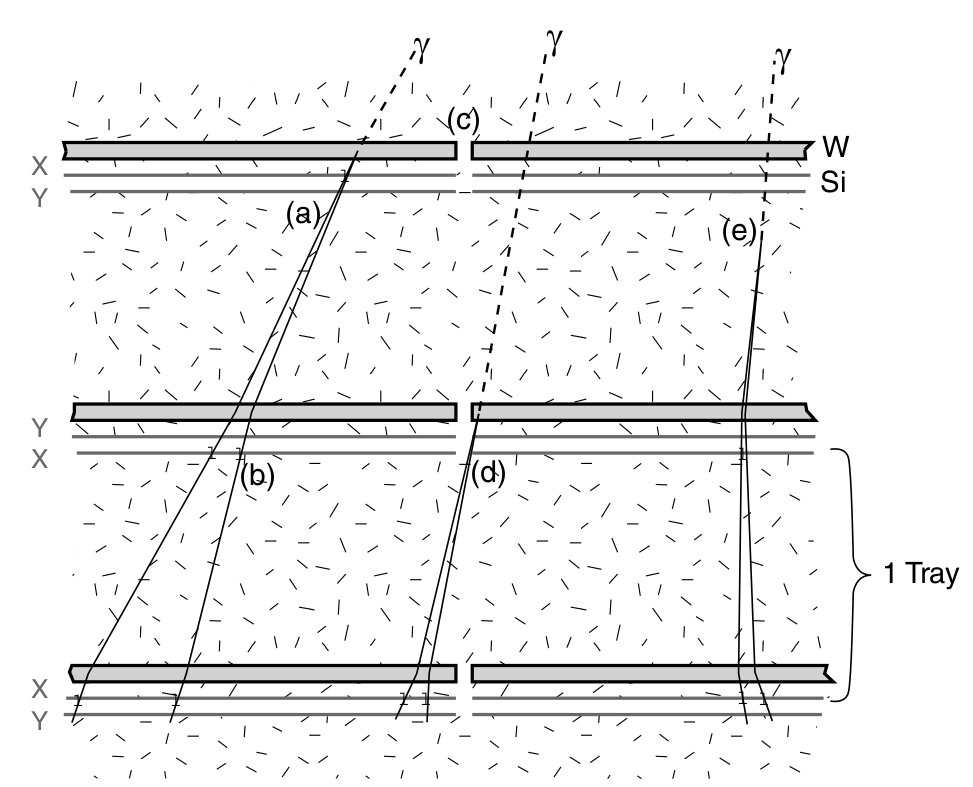
\includegraphics[width=0.6\textwidth]{content/background/figures/fermi_tracker.png}
    \caption{LAT's particle tracker (Image taken from \cite{FermiLAT})}
    \label{fig:fermi_tracker}
\end{figure}

The particle tracking is made from silicon-strip. Tracking information 
would leave the track in 2-D plane of a particle tracking. In order to
trace back and gaining data as the 3-D moving direction, 16 particle 
tracker has to be taken in account for constructing the electron 
or positron path.
Despite one layer of particle tracking could obtain 
the information about incoming leptons for x-y plane only, but techinical 
design of LAT does put a 2 layers of silicon-based tracker with a very 
narrow gap between them. This kind of design could make the LAT performing 
measurement precision in the angular resolutiom better than a single 
layer of a wide gap which affects in the point-spread function (PSF)
of the probability distribution from reconstruction direction.
According to Figure \ref{fig:fermi_tracker}, top and the bottom of
silicon trackers and the heavy-nuclei conversion layer called "Tray".
Case (a) and (b) in the figure is the ideal case where the $\gamma$-ray
hit the conversion layer and multiple footprints are recorded.
Nevertheless, there is an edge case as in (d) and (e) where the $\gamma$-ray
has a probability to skip an early layer and choose to covert in the 
secondary conversion layer and will be detected in the upcoming 
tracking layer. The major benefit of deploying multiple conversion 
layers is quite obvious for the better event gathering.


\subsubsection{Calorimeter}
Unlike particle tracker that talk to a charged particle by utilizing
the EM induction without (or barely) disturbing the particle state,
calorimeter is a starving component. It consume a lepton and produce 
electronic readout of the energy from radiation of the lepton in the
crystal scintillator. Definitely, size of this part is mainly considered 
from the radiation lengths of the electron and position particles becasue it 
has to record the shower that happen during the decaying process.
However, the radiation length highly depends on the kinetic energy 
of the particle. The LAT itself has been designed for detecting photon 
energy range between MeV to a few hundred GeV. Hence, the exposure of 
photon energy beyond TeV is probably not promising in this case.


\begin{figure}[h]
    \centering
    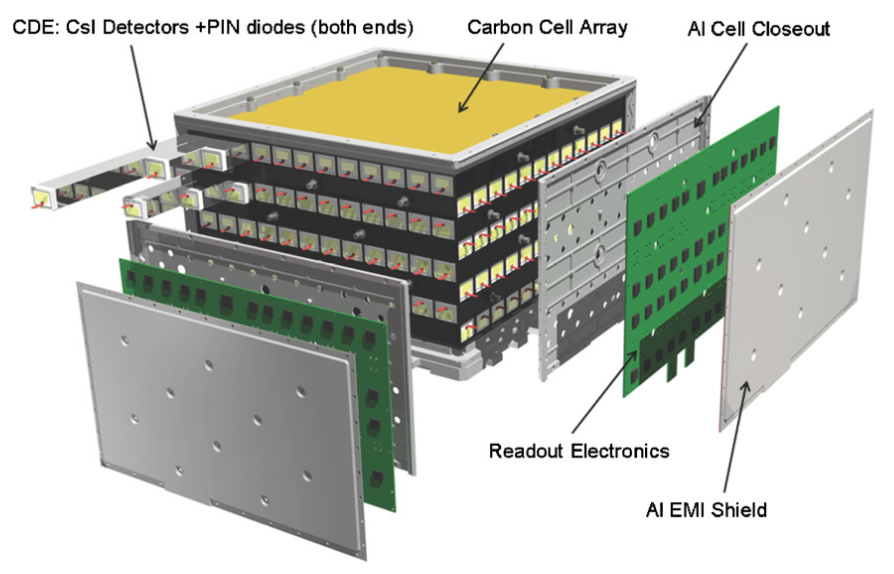
\includegraphics[width=0.8\textwidth]{content/background/figures/fermi_calorimeter.png}
    \caption{LAT's calorimeter (Image taken from \cite{FermiLAT})}
    \label{fig:fermi_calorimeter}
\end{figure}

The overview apparatus structure is illustrate in Figure \ref{fig:fermi_calorimeter}.
Each calorimeter module consists of 96 CsI(Tl) scintillator crystal size 
2.7 cm x 2.0 cm x 32.6 cm and PIN photodiodes at both ends which connect 
to the readout electronic components for translate an amount of light 
that has been sparked in the crystal to digitized signal. Each horizontal 
layer is combined from 12 crystal component and stack them 8 times by 
rotate them 90\textdegree each for boosting the angular resolution 
from the sparking lights. The carbon cell was build for supporting 
the structure of low mass particle tracker due to the properties of 
high stiffness, thermal conductivity and thermal stability.
An electron, position or $\gamma$-ray will deposit the energy in the
calorimeter as the scintillated lights via electromagnetic intereaction.
The segmented crystal also allow LAT to trace the shower
as the spatial imaging.


\subsubsection{Anti-coincidence Detector (ACD)}
The main objective of ACD is to support the charged-particle background 
rejection of the CRs. It is cover the tracker over the LAT field of 
view (FoV) for 4 side and the top part of the LAT. It consists of 
89 plastic scintillator tiles with 5 $\times$ 5 array on top and 
4 sides of 16 tiles. Each tile component contains two photomultiplier 
and wanelength shifting fibers embedded in the scintillator. The tile 
is overlapping another one in one-dimension to reduce the effect of 
the gaps between them. To be more prcise, there are two sets 
of four called scintillator ribbon for covering the top-down side 
and a pair around their center. The ACD is required to has 0.9997 efficientcy 
for detecting an incoming charged particle of FoV of the LAT. However,
the $\gamma$-ray induce the shower that calorimeter will absorb but 
there is a scenario called "backsplash effect" where the secondary 
particles in keV range from the electromagnetic shower could interact 
with the incoming photon and Compton scattering in ACD. Then it could 
create a veto signal from the recoil electron. In order to solve this issue,
the ACD with their neighborhood would take the incident candidate photon 
into account and could dramatically reduce the effect of the backsplashing.


\subsubsection{Data Acquisition System (DAQ)}


To acquire an interesting event, event selection could not be done 
on software on the ground level from the whole raw signal of subsystems because the limitation 
of the hardware in the current edge. In order to collect an event, 
raw data will be selected from filtering algorithm on board.
The hierarchical structure of data acquisition system (DAQ) was invented 
for seeking an transient event as shown in Figure \ref{fig:fermi_daq}.

\begin{figure}[h]
    \centering
    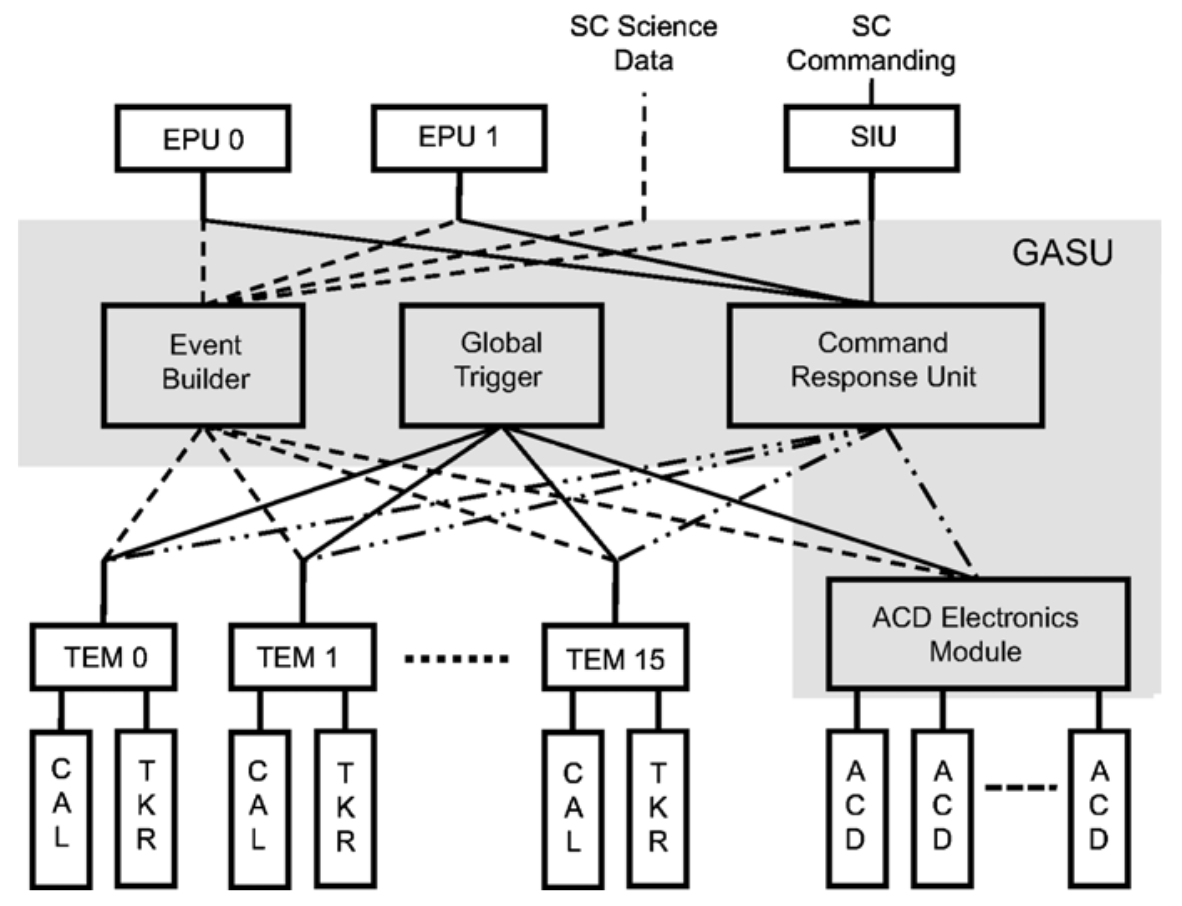
\includegraphics[width=0.6\textwidth]{content/background/figures/fermi_daq.png}
    \caption{Flow chart of LAT's data acquisition system (DAQ) (Image taken from \cite{FermiLAT})}
    \label{fig:fermi_daq}
\end{figure}

The lowest level is tower electronic modules (TEMs) to serve as an 
interface for the tracker and calorimeter. All TEMs create event 
buffering and communicates with Event Builder Module (EBM) which is a
component of Global-trigger/ACD-module/Signal distribution Unit (GASU).
Command Response Unit (CRU) was built to communicate the
software execution in DAQ system. Lastly, Event Processing Unit (EPU)
will process a selecting event from TEM and ACD Electronics Module (AEM).
Filtering an event could reduce the information flowing rate from 
a few kHz to around 400 Hz which will be sent back to the ground level.


\subsection{Event reconstruction}

In an early day, the reconstruction algorithm for tracing a photon 
is Monte Carlo (MC) simulation. Modeling the incident $\gamma$-rays 
and the background has been simulated in the orbiting-like environment 
before it launch. Meaning that background rejection property already 
embedded in the LAT since the developing process. The simulation 
could be use for the detector calibration since the simulation software 
provide an interaction physical process.

The main logic of the reconstruction is started by tracking the footprint 
in the tracker and expect the output in calorimeter cube as physical process 
would yield. After that the event classificaiton mainly consider from 
the ACD part to classify an event types.

The result from processed data on the fly is level 0 and it will pass 
down to Earth and reconstructing the photon data called level 1.
The more LAT orbiting around the Earth's, the more understanding of the 
LAT environment and it brings the software improvement for the reconstruction
algorithm to exploid the technique of pattern recognitions.
First official released is LAT data is Pass 6 and Pass 7 after has been 
released with the same level 0 data but the reconstructed event is 
more efficient than the older one by software level. The newest version 
and likely to be the final version is Pass 8. Not only the reconstruction
algorithm that has been devided but the event class is also an 
crucial concept. As mentioned earlier, the photon is clsssified into 
a specific class. There is no free lunch to think that the detector see 
the particle as a binary classificaiton. It will mix with a likelihood 
or probability to distinguish the specific kind of interesting event.
That is the main reason why \textit{Fermi}-LAT team split the event 
into multiple classes which mainly are TRANSIENT, SOURCE, ULTRACLEAN and 
ULTRACLEANVETO.

Definitely, lesser photon candidates has been selected in 
the ULTRACLEANVETO. Then there is no certain right or wrong for
picking the class from researcher point of view. The main criteria 
would be the objectives of the analysis. If the analyzer want a 
huge events and could accept some noisy event, then SOURCE or 
TRANSIENT class is suitable for the analysis and vice versa.


\subsection{Detector performance and their characteristics}

\begin{figure}[h]
    \centering
    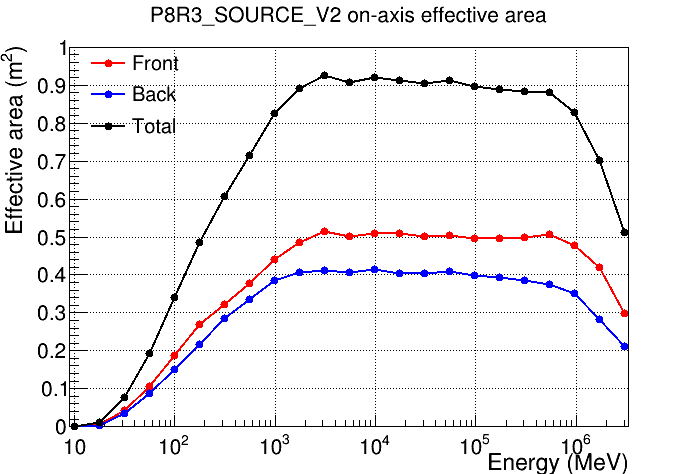
\includegraphics[width=0.7\textwidth]{content/background/figures/eff_energy.png}
    \caption{
        Effective area along the photon energy range from MeV to TeV
        (\cite{lat_p8_performance})
    }
    \label{fig:eff_energy}
\end{figure}

\textit{Fermi}-LAT has been designed for detecting $\gamma$-ray in the 
space which means that the range of energy that it could see precisely 
will starting at MeV up to TeV. The effective area in square-meters
is defined from the front and the back of the LAT's tracking layer 
by consider the upper part as a front and the bottom part belowing 
a certain layer as the back part. Since both front and back part 
components is made by the same materials and exactly same design. 
Then total effective area could be sum into a single value. 
The Figure \ref{fig:eff_energy} visualize the effectiveness of LAT 
along a given energy range. According to the plot, LAT performs 
a measurement well from GeV up to TeV scale.


Another crucial part when dealing with LAT effectiveness is the 
incidence angle ($\theta_\text{LAT}$). It highly affects to the 
number of tracking layers. The higher probability of passing more 
tracking layers would yield a better LAT's performance. Figure 
\ref{fig:eff_theta} shows relation of effective area versus 
incidence angle.


% angle dependency 
\begin{figure}[h]
    \centering
    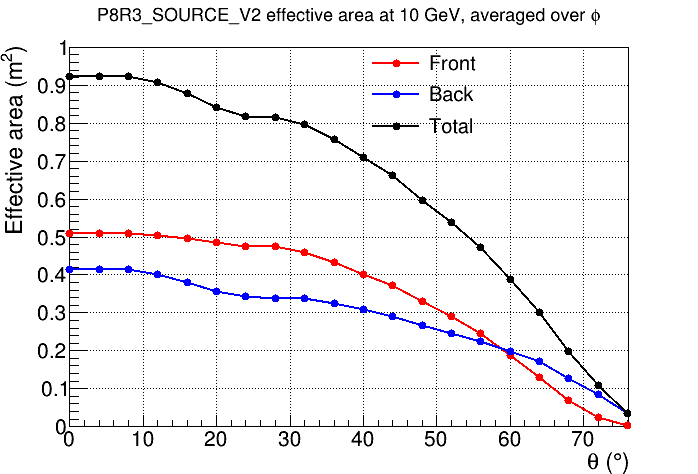
\includegraphics[width=0.7\textwidth]{content/background/figures/eff_theta.png}
    \caption{Effective area versus incidence angle (\cite{lat_p8_performance})}
    \label{fig:eff_theta}
\end{figure}

Imagine the LAT structure as a cube-like detector. Surely, the LAT 
boresight is a square where an azimuthal angle ($\phi_\text{LAT}$) of the incoming 
photon would affect a larger area that the photon could intereact 
as demonstrates in Figure \ref{fig:eff_theta}. The reason why there 
is a peak for any cycle of $\pi/2$ radian or 90\textdegree is 
the edge of the LAT would has more area to interact than the 
lateral. Another evidence for the explaination is the front effective 
area has less effects since the propagation length is narrow than 
the back.

\begin{figure}[h]
    \centering
    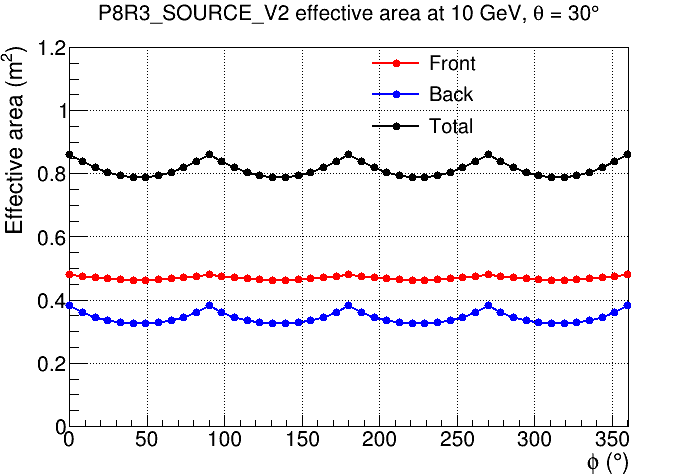
\includegraphics[width=0.7\textwidth]{content/background/figures/eff_phi.png}
    \caption{Effective area versus azimuthal angle (\cite{lat_p8_performance})}
    \label{fig:eff_phi}
\end{figure}

% event class
\begin{figure}[h]
    \centering
    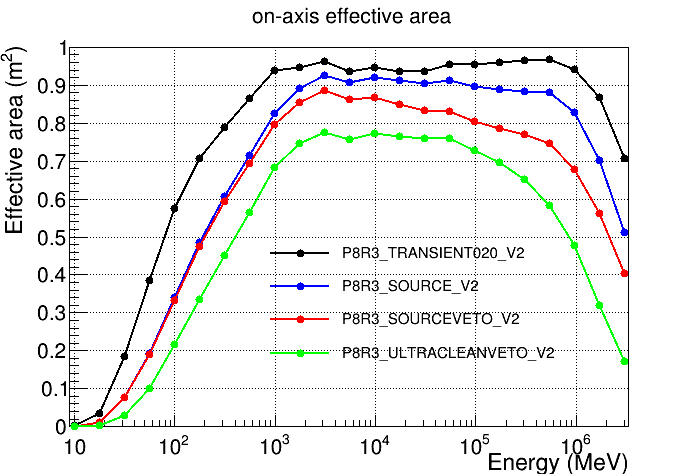
\includegraphics[width=0.7\textwidth]{content/background/figures/eff_event_class.png}
    \caption{Effective area along the energy of each event class (\cite{lat_p8_performance}))}
    \label{fig:eff_event_class}
\end{figure}


From the previous subsection, the event class is also play crucial 
role when considering the effectiveness of the reconstructed event.
Undoubtly, the cleanest class namely "ULTRACLEANVETO" would has 
the worst effective area. In opposite, TRANSIENT class would yield 
the best effective area as visualized in Figure \ref{fig:eff_event_class}.

To sum up, the effective area act for the LAT performance for seeking 
an event in the unit of square lengths. It is also behave like a function 
in the practical analysis which pragmatically allow the client to 
throw incidence angle, azimuthal angle and the energy. Then it will 
return the effective area in unit of square centi-meters in the raw 
format.